\section{Linux}
\subsection{Storia}
Negli anni '40 e '50 i computer venivano spesso condivisi tra diversi utenti in quanto essi erano pricipalmente utilizzati da ricercatori per i loro calcoli.
Per questo motivo vengono inventati dei sistemi operativi adatti a gestire il time sharing di più utenti, \textbf{MULTICS} è uno di essi, sviluppato dai ricercatori di MIT, Bell Labs e General Electric.

\spacer
Uno dei ricercatori di Bell Labs, Ken Thompson, iniziò a scrivere una versione ridotta di MULTICS, adatta a gestire solamente un utente, per questo motivo venne chiamato ironicamente \textbf{UNICS}.

\subsubsection{Porting}
Nel tempo questo sistema operativo viene portato su diversi computer, per rendere più agevole il processo si cerca di riscriverlo in un linguaggio ad alto livello.
Inizialmente Bell Thompson crea il linguaggio \textbf{B}, una semplificazione del BCPL, ma non riesce a portare a termine questo progetto a causa di alcune debolezze del B (in particolare la sua mancanza di struct).

Con l'aiuto di Ritchie progetta quindi un successore al B, chiamandolo (ovviamente) \textbf{C}, con il quale riescono a riscrivere UNIX in un linguaggio ad alto livello.

Dopo la scrittura in C altro lavoro deve essere fatto per rendere UNIX facilmente portabile, si è scoperto infatti che il sistema faceva alcune assunzioni riguardo all'hardware su cui veniva eseguito.

\subsubsection{Separazione e riconciliazione}
La licenza per UNIX, assieme al suo codice sorgente, venero forniti facilmente a diverse università, le quali continuarono il lavoro iniziato e distribuirono ulteriormente il sistema operativo.

In particolare la versione sviluppata all'università di Berkley ha ricevuto parecchi miglioramenti rispetto alla versione di Bell Labs, rendendola la versione più popolare negli ambienti accademici.

\spacer
A questo punto le versioni dei UNIX si sono però divise e i programmi non sono interscambiabili, rendendo difficile la distribuzione di software.
Per ovviare al problema l'IEEE fornisce uno standard di procedure di libreria che ogni sistema operativo avrebbe dovuto supportare, esso viene chiamato \textbf{POSIX}.

\subsubsection{MINIX}
\textbf{MINIX} è un'altro sistema operativo nato dal codice sorgente di UNIX, ma viene creato con l'obbiettivo di ottenere le massime prestazioni e di essere interamente comprensibile da un singolo sviluppatore.

\spacer
Questo ha portato MINIX ad essere estreamente limitato e quando gli utenti chiedevano se fosse possibile aggiungere certe funzionalmente si sentivano rispondere di no perché il codice sarebbe diventato troppo grande.

\subsubsection{Linux}
Questi continui "no" hanno portato molti utenti a cercare un'alternativa, e la trovarono in \textbf{Linux}, un sistema operativo sviluppato da uno studente finlandese, Linus Torvalds.

Il codice di questo sistema operativo esplode rapidamente con molti utenti felici di contribuire con le loro migliorie, arrivando a Linux 5.11 dove il kernel è composto da 30 milioni di righe di codice.

Linux nel tempo è rimasto un software libero, il cui codice sorgente può essere letto e modificato da tutti. Esso è coperto dalla licenza \textbf{GPL} che specifica cosa può essere fatto e cosa no, in particolare non è possibile modificare il codice e redistribuirlo solamente in forma binaria.

\subsubsection{Obiettivi}
Linux viene concepito come un sistema operativo scritto da programmatori, per programmatori. Fornendo quindi un sistema semplice, elegante e coerente.

Altre caratteristiche importanti per i programmatori sono il "principio della minima sorpresa", potenza, flessibilità e assenza di rindondanza.

\subsection{Processi}
Ogni processo in linux viene rappresentato attraverso una task\_struct che contiene tutte le informazioni.

\subsubsection{Deamon}
I deamon sono dei processi di background che vengono eseguiti periodicamente.

\subsubsection{Fork}
La chiamata a sistema fork è di particolare importanza, essa permette di creare una copia esatta del processo su cui viene chiamata.

Essa ritorna l'id del processo figlio al genitore e ritorna 0 al figlio, questo permette di distinguere il contesto.

\begin{minted}{c}
pid = fork();
if (pid < 0) {
    handle error();
} else if (pid > 0) {
    /* codice genitore qui.*/
} else {
    /* codice figlio qui.*/
}
\end{minted}

I figli utilizzano la tecnica del copy on write per non creare troppo overhead alla creazione di un nuovo thread.

\subsubsection{Clone}
Una funzione introdotta nel 2000 è clone, la quale ha sfumato la distinzione tra processo e thread. Infatti grazie a questa system call è possibile specificare quali informazioni del genitore devono essere condivisi al figlio e quali no.

\subsubsection{Comunicazione}
Per la comunicazione tra processi è possibile utilizzare delle \textbf{Pipe}, oppure degli interrupt software, detti \textbf{Signal}.

\subsection{Scheduling}
Le politiche implementate da linux sono:
\begin{sitemize}
    \item \textbf{Real Time FIFO:} priorità massima, non possono essere prelati se non da altri processi a priorità maggiore.
    \item \textbf{Real Time Round Robin:} alta priorità, vegnono prelati solo da processi a priorità maggiore o quando termina il quanto di tempo.
    \item \textbf{Sporadici:} bassa priorità, vengono eseguiti quando ci sono delle risorse libere.
    \item \textbf{Time Sharing:} priorità minima, vengono eseguiti con priorità minore di quelli sporadici.
\end{sitemize}

\spacer
Le categorie Real Time condividono le priorità 0-99, le altre due le priorità 100-139.
La priorità può anche essere modificata da un valore "cortese" (nice), che ha valore da -20 a +19. Un processo che sa di essere a bassa priorità può ridurla tramite una chiamata a sistema.

\spacer
Queste politiche vengono implementate dal \textbf{CFS} (\textit{Completely Fair Scheduler}), il quale cerca di dare a tutti i processi lo stesso tempo di CPU.
Per implementare la priorità la valocità effettiva del tempo viene modificata, è più lenta per i processi ad alta priorità e più veloce per quelli a bassa priorità.

\subsection{Avvio}
Il bootloader di default di Linux è  \textbf{GRUB} (GRand Unified Bootloader), a seguito viene avviato il kernel.

Esso inizializza prima l'hardware (identificazione tipo CPU, RAM, attivazione MMU, disattivazione interrupt), e successivamente il software (allocazione buffer dei messaggi, strutture dati kernel, configurazione dei dispositivi I/O).

Poi viene creato il processo 0 il quale svolge altre inizializzazioni software e poi crea il processo 1 (init) e il processo 2 (page deamon).

Infine viene eseguito un programma chiamato getty che mostra all'utente una schermata di login.

\subsection{Gestione della Memoria}
In linux su sistemi a 64 bit vengono utilizzati solo 48 per l'indirizzamento della memoria principale, fornendo così un limite teorico di 258 Tb di memoria, e 128 Tb per ogni processo.

\spacer
Le architetture degli elaboratori suddividono la memoria in diverse aree:
\begin{sitemize}
    \item ZONE\_DMA
    \item ZONE\_NORMAL
    \item ZONE\_HIGHMEM che non viene mappata in modo permanente
\end{sitemize}

\spacer
Linux per indicizzare la memoria utilizza uno schema di paginazione a 4 livelli

\begin{figure}[H]
    \centering
    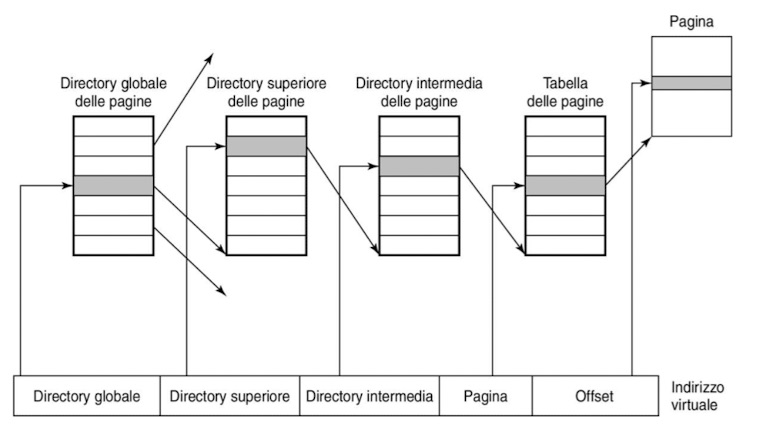
\includegraphics[width=0.5\linewidth]{assets/linux-pager.jpeg}
\end{figure}

\subsubsection{Allocatore}
L'allocatore di memoria utilizzato da linux è una combinazione dell'algoritmo Buddy (potenza a 2) e un algoritmo slab.

La memoria viene prima suddivisa dall'algoritmo buddy, poi le varie zone sono gestite dall'algoritmo slab.

\subsubsection{Paginazione}
La memoria viene paginata solamente su richiesta, l'algoritmo di reclamo delle pagine suddivide le pagine in 4 categorie:

\begin{sitemize}
    \item \textbf{unreclaimable} Pagine bloccate e non recuperabili.
    \item \textbf{swappable} Pagine che devono essere scritte sulla zona di swap del disco prima di poter procedere.
    \item \textbf{syncable} Pagine il cui contenuto è stato modificato, quindi devono essere riportate sul disco.
    \item \textbf{discarable} Pagine che possono essere eliminate direttamente.
\end{sitemize}

\subsubsection{I/O}
I dispositivi I/O vengono trattati da linux come dei \textbf{file speciali}, montati nel file system virtuale.

\spacer
Essi sono divisi in due tipologie:
\begin{sitemize}
    \item \textbf{file speciali a blocchi:} sequenze di blocchi numerati ad accesso causale, ideali per i dischi.
    \item \textbf{file speciali a caratteri:} flusso di caratteri, utili per tastiere e stampanti.
\end{sitemize}

\spacer
Il networking viene implementato mediante dei socket che permettono al sistema di interfacciarsi ad un cavo.

\begin{figure}[H]
    \centering
    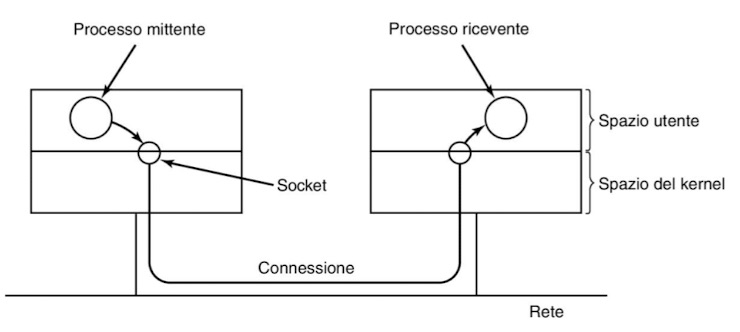
\includegraphics[width=0.5\linewidth]{assets/linux-socket.jpeg}
\end{figure}

Ogni socket supporta un particolare tipo di rete:
\begin{sitemize}
    \item flusso di byte con connessione affidabile (TCP)
    \item flusso di pacchetti con connessione affidabile
    \item flusso di pacchetti con connessione non affidabile (UDP)
\end{sitemize}

\subsubsection{File System}

\subsubsection{ext2}
Il primo file system implementato da linux è ext2, il quale suddivide il disco in blocchi, ognuno dei quali ha una sezione detta \textbf{superblocco} che contiene informazioni sulla struttura della sezione.
Poi contiene due bitmap, una per i blocchi liberi e una per gli i-node liberi.
Infine vengono salvati i blocchi e gli i-node.

\begin{figure}[H]
    \centering
    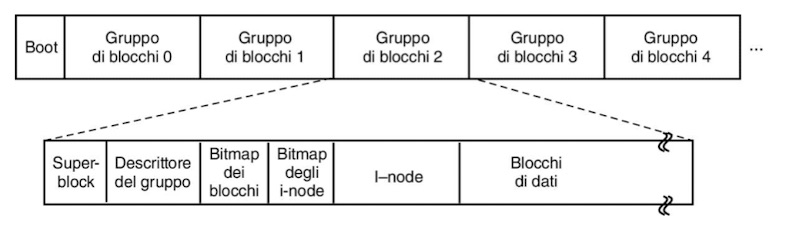
\includegraphics[width=0.5\linewidth]{assets/linux-ext2.jpeg}
\end{figure}

\subsubsection{ext4}
Il file system ext4 introduce il jounaling, ovvero le istruzioni vengono salvate dal sistema operativo prima di essere inviate al disco e vengono eliminate quando completate.

Questo significa che in caso di terminazione inaspettata il sistema può riportare il disco allo stato atteso.

\subsection{Sicurezza}
In linux la sicurezza e la condivisione vengono implementate mediante un id dell'utente e un id del gruppo.
Ogni file è contrassegnato dall'identificativo dell'utente e del gruppo proprietari.

\spacer
A questo punto è sufficiente specificare con 9 bit i permessi, 3 per il proprietario, 3 per il gruppo e 3 per gli esterni.

I 3 bit sono:
\begin{sitemize}
    \item read
    \item write
    \item execute
\end{sitemize}
